%%%% SELECT ONE OF THE FOLLOWING COMMANDS %%%%%%%%

%%% TEMPLATE FOR PROCEEDINGS TRACK %%%%
\documentclass[mlmain]{jmlr}

%% TEMPLATE FOR Extended Abstract Track %%%%%%%
% \documentclass[mlabstract]{jmlr}

%%%%%%%%%%%%%%%%%%%%%%%%%%%%%%%%%%%%%%%%%%%%%%%%%

% ------------------------
% Course report note:
% This template includes a review watermark by default. For this course report
% (not an anonymous workshop submission), we disable the watermark.
% ------------------------


   
% The following packages will be automatically loaded:
% amsmath, amssymb, natbib, graphicx, url, algorithm2e


%%% WARNING %%%%
%%% 1) Please, use the packages automatically loaded to manage references, write equations, and include figures and algorithms. The use of different packages could create problems in the generation of the camera-ready version. Please, follow the examples provided in this file.
%%% 2) References must be included in a .bib file.
%%% 3) Write your paper in a single .tex file.
%%%

%%%% SOFTWARE %%%%
%%% Many papers have associated code provided. If that is your case, include a link to the code in the paper as usual and provide a link to the code in the following comment too. We will use the link in the next comment when we generate the proceedings.
%%% Link to code: http://?? (only for camera ready)

 %\usepackage{rotating}% for sideways figures and tables
\usepackage{longtable}% for long tables

 % The booktabs package is used by this sample document
 % (it provides \toprule, \midrule and \bottomrule).
 % Remove the next line if you don't require it.
\usepackage{booktabs}
 % The siunitx package is used by this sample document
 % to align numbers in a column by their decimal point.
 % Remove the next line if you don't require it.
\usepackage[load-configurations=version-1]{siunitx} % newer version
 %\usepackage{siunitx}

% Prevent figures/tables from appearing before their definition.
\usepackage{flafter}
% Allow forcing floats to appear "here".
\usepackage{float}

% Prepend the SCUT course-report cover page (built separately with XeLaTeX).
\usepackage{pdfpages}

% Hide colored link borders/colors in the PDF (still clickable).
\hypersetup{hidelinks}

% Space saving for course-page limits.
\setlength{\abovedisplayskip}{4pt}
\setlength{\belowdisplayskip}{4pt}
\setlength{\abovedisplayshortskip}{2pt}
\setlength{\belowdisplayshortskip}{2pt}
\setlength{\itemsep}{2pt}
\setlength{\topsep}{2pt}
\setlength{\parskip}{0pt}
\setlength{\abovecaptionskip}{3pt}
\setlength{\belowcaptionskip}{0pt}

% Make figure captions slightly smaller and more compact.
\makeatletter
\renewcommand{\fnum@figure}{\footnotesize Figure \thefigure}
\makeatother

 % The following command is just for this sample document:
\newcommand{\cs}[1]{\texttt{\char`\\#1}}

 % Define an unnumbered theorem just for this sample document:
\theorembodyfont{\upshape}
\theoremheaderfont{\scshape}
\theorempostheader{:}
\theoremsep{\newline}
\newtheorem*{note}{Note}

%%%% DON'T CHANGE %%%%%%%%%
\jmlrvolume{}
\firstpageno{1}
\editors{}

\jmlryear{2026}
\jmlrworkshop{084100291 Matrix Analysis and Computation}

%\editor{Editor's name}
%%%%%%%%%%%%%%%%%%%%%%%%%%%



\title[Reproducing PiSSA]{Reproducing PiSSA: Principal Singular Values and Singular Vectors Adaptation of Large Language Models --- A Reproduction Study}

%%%%%%%%%%%%%%%%%%%%%%%%%%%%%%%%%%%%%
% THE MANUSCRIPT, DATA AND CODE MUST BE ANONYMIZED DURING THE REVIEW PROCESS. 
% DON'T INCLUDE ANY INFORMATION ABOUT AUTHORS DURING THE REVIEW PROCESS.
% Information about authors (Full names, emails, affiliations) have to be provided only for the submission of the camera-ready version.  Only in that case, you can uncomment and use the next blocks.
%%%%%%%%%%%%%%%%%%%%%%%%%%%%%%%%%%%%%

 % Use \Name{Author Name} to specify the name.

 % Spaces are used to separate forenames from the surname so that
 % the surnames can be picked up for the page header and copyright footer.
 
 % If the surname contains spaces, enclose the surname
 % in braces, e.g. \Name{John {Smith Jones}} similarly
 % if the name has a "von" part, e.g \Name{Jane {de Winter}}.
 % If the first letter in the forenames is a diacritic
 % enclose the diacritic in braces, e.g. \Name{{\'E}louise Smith}

 % *** Make sure there's no spurious space before \nametag ***

 % Two authors with the same address
%   \author{\Name{Author Name1\nametag{\thanks{with a note}}} \Email{abc@sample.com}\and
%   \Name{Author Name2} \Email{xyz@sample.com}\\
%   \addr Address}

  %Three or more authors with the same address:
%   \author{\Name{Author Name1} \Email{an1@sample.com}\\
%   \Name{Author Name2} \Email{an2@sample.com}\\
%   \Name{Author Name3} \Email{an3@sample.com}\\
%   \Name{Author Name4} \Email{an4@sample.com}\\
%   \Name{Author Name5} \Email{an5@sample.com}\\
%   \Name{Author Name6} \Email{an6@sample.com}\\
%   \Name{Author Name7} \Email{an7@sample.com}\\
%   \Name{Author Name8} \Email{an8@sample.com}\\
%   \Name{Author Name9} \Email{an9@sample.com}\\
%   \Name{Author Name10} \Email{an10@sample.com}\\
%   \Name{Author Name11} \Email{an11@sample.com}\\
%   \Name{Author Name12} \Email{an12@sample.com}\\
%   \Name{Author Name13} \Email{an13@sample.com}\\
%   \Name{Author Name14} \Email{an14@sample.com}\\
%   \addr Address}


 % Authors with different addresses:
 % \author{\Name{Author Name1} \Email{abc@sample.com}\\
 % \addr Address 1
 % \AND
 % \Name{Author Name2} \Email{xyz@sample.com}\\
 % \addr Address 2
 %}

% Course report author block (non-anonymous).
\author{\Name{Xiangyun Xiao} \Email{ftxiaoxiangyun@mail.scut.edu.cn}\\
\addr South China University of Technology\\
084100291 Matrix Analysis and Computation, Spring 2026}



\begin{document}

% SCUT cover page as page 1 (compile cover/cover.tex with XeLaTeX first).
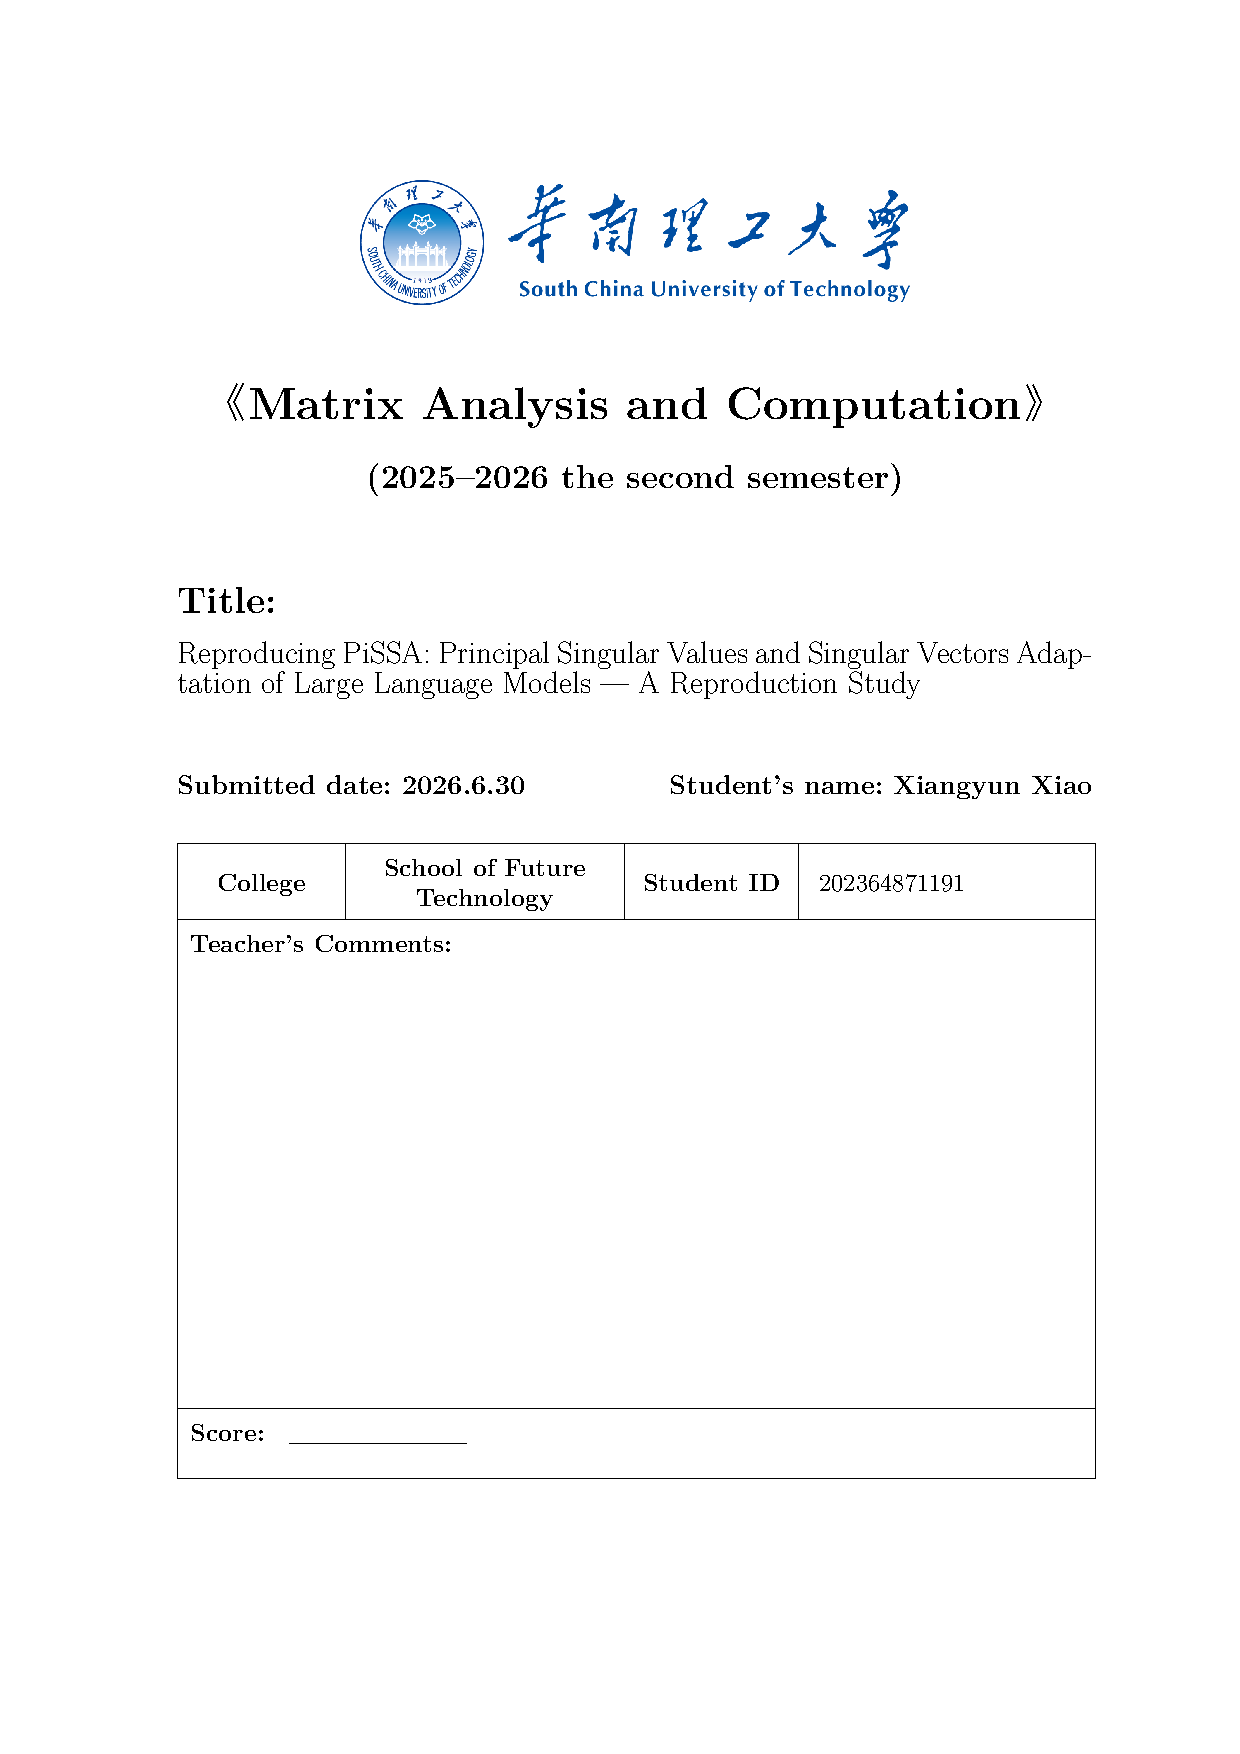
\includepdf[pages=1,fitpaper=true]{cover/cover.pdf}

\maketitle

% Override running headers (even/odd pages) for course report.
\markboth{Reproducing PiSSA}{Reproducing PiSSA}

\begin{abstract}
Parameter-efficient fine-tuning (PEFT) makes adapting large language models (LLMs) affordable. The widely used Low-Rank Adaptation (LoRA) initializes its adapter with Gaussian noise and zeros, so the injected update is zero at the start of training, which can slow convergence. PiSSA \citep{meng2024pissa} instead initializes the adapter from the \emph{principal} singular components of the pretrained weight and freezes the residual, claiming faster convergence and accuracy on par with full fine-tuning. In this work we independently reproduce PiSSA from scratch (without the official PEFT integration) and stress-test its central claims. On LLaMA-2-7B fine-tuned on MetaMathQA and evaluated on GSM8K, our reproduced PiSSA matches full fine-tuning exactly (39.88\% vs.\ 39.88\%) and clearly outperforms LoRA (32.37\%, $+7.5$ points), faithfully reproducing the paper's main ordering PiSSA~$\ge$~Full~$>$~LoRA. We further reproduce, with our own NF4 implementation, that PiSSA decomposition reduces the 4-bit quantization error of the frozen residual, and we recover the paper's exact per-projection pattern (attention $Q/K$ benefit most, MLP projections least). We extend the study across four heterogeneous architectures (ChatGLM3, Qwen2.5, LLaMA-3, Baichuan2). Where our numbers diverge from the original paper---notably a lower absolute quantization-error reduction and a QPiSSA training result below QLoRA---we report the discrepancies honestly and attribute them to implementation and compute-budget differences rather than to a failure of the method.
\end{abstract}
\begin{keywords}
Parameter-efficient fine-tuning; LoRA; singular value decomposition; 4-bit quantization; reproducibility
\end{keywords}

\section{Introduction}
\label{sec:intro}
Fine-tuning large language models (LLMs) in full precision is expensive in both memory and compute, which has motivated a family of parameter-efficient fine-tuning (PEFT) methods. Among them, Low-Rank Adaptation (LoRA) \citep{hu2022lora} is the most widely adopted: it freezes the pretrained weight $W$ and learns a low-rank update $\Delta W = AB$ with $A$ drawn from Gaussian noise and $B$ set to zero, so that $AB = 0$ at initialization and the model output is unchanged at the start of training. A side effect of this ``noise-and-zero'' initialization is that the early gradients can be small or poorly directed, leading to slow convergence and, occasionally, a worse local optimum.

PiSSA (Principal Singular values and Singular vectors Adaptation) \citep{meng2024pissa} keeps the LoRA architecture but changes the initialization: it applies a singular value decomposition (SVD) to $W$, uses the top-$r$ \emph{principal} components to initialize the trainable adapter $A,B$, and freezes the remaining \emph{residual} components $W^{res}$. Because the principal components capture the directions in which $W$ acts most strongly, PiSSA is claimed to converge faster and to reach accuracy comparable to full fine-tuning, while its 4-bit variant QPiSSA quantizes only the (narrower-spectrum) residual and therefore incurs a smaller quantization error than QLoRA.

The appeal of PiSSA is twofold and worth stating precisely. First, it promises to close the long-standing accuracy gap between low-rank adaptation and full fine-tuning without adding any inference-time cost, since the adapter can be merged back into the weight after training. Second, by operating on the weight rather than the update, it offers a principled, data-free initialization: the decomposition depends only on the pretrained weight and can be computed once, offline. These properties make PiSSA an attractive default, but they also raise the stakes for reproduction---if the principal-component initialization is truly the deciding factor, the effect should appear consistently across architectures and should survive an implementation that shares no code with the original release. This is precisely the kind of claim a from-scratch reproduction is well suited to test.

Reproducibility is a cornerstone of empirical machine learning. The goal of this work is not to propose a new method but to \emph{independently verify} the central claims of PiSSA, and to be explicit about where a from-scratch reproduction agrees or disagrees with the original report. We take the position that a reproduction is successful when (i) the method is implemented faithfully, (ii) all results are reported honestly regardless of whether they confirm the original, and (iii) discrepancies are given a credible attribution. Our contributions are:
\begin{itemize}\setlength{\itemsep}{1pt}
\item A from-scratch implementation of PiSSA and QPiSSA (SVD initialization, residual freezing, and a custom NF4 residual layer), validated for numerical correctness (Section~\ref{sec:m0}).
\item A reproduction of the core LLaMA-2-7B / MetaMathQA / GSM8K benchmark, where PiSSA matches full fine-tuning and beats LoRA, together with a side-by-side comparison against the numbers reported in the original paper (Sections~\ref{sec:m1} and \ref{sec:discussion}).
\item A cross-architecture generality probe over ChatGLM3-6B, Qwen2.5-7B, LLaMA-3-8B, and Baichuan2-7B (Section~\ref{sec:m2}).
\item An NF4 quantization study (QPiSSA vs.\ QLoRA): a paper-aligned per-projection error-reduction table and an end-to-end training comparison, with an honest analysis of where and why our results differ (Section~\ref{sec:m3}).
\end{itemize}

\section{Background and Related Work}
\label{sec:related}
\paragraph{Low-rank adaptation.} LoRA \citep{hu2022lora} reparameterizes the weight update as a product of two low-rank matrices, reducing the number of trainable parameters by orders of magnitude while preserving inference speed after merging. Numerous variants adjust the rank adaptively or refine the update direction. PiSSA differs philosophically: rather than approximating the \emph{update} $\Delta W$, it decomposes the \emph{weight} $W$ and fine-tunes its principal part. A second, often overlooked consequence of LoRA's initialization is that its two factors play asymmetric roles---one is random and one is exactly zero---so the earliest updates are driven entirely by the random factor while the zero factor receives gradient only indirectly. PiSSA removes this asymmetry by giving both factors a meaningful, weight-derived starting point. Most other variants keep the random-update philosophy and intervene on the rank schedule, the scaling factor $\alpha$, or where adapters are placed; PiSSA is distinctive in that its initialization is fully determined by the pretrained weight and requires no training data to compute.

\paragraph{Quantized fine-tuning.} QLoRA \citep{dettmers2023qlora} combines LoRA with 4-bit NormalFloat (NF4) quantization of the base model, enabling memory-efficient fine-tuning while keeping the adapter in higher precision. LoftQ \citep{li2023loftq} reduces the quantization error by absorbing part of it into the adapter initialization. QPiSSA reduces quantization error differently: it quantizes the residual $W^{res}$, whose singular spectrum is narrower than that of $W$, and is therefore more amenable to NF4.

\paragraph{Why principal components help.} The singular value decomposition orders the directions of $W$ by how strongly the linear map stretches its input. LoRA's random initialization places the trainable subspace at an arbitrary, typically low-energy orientation, so early optimization must first rotate the adapter toward useful directions before it can make real progress. PiSSA instead seeds the adapter with the highest-energy directions, which the original work argues yields gradients that resemble those of full fine-tuning from the first step. The same decomposition explains the quantization benefit: removing the few dominant singular values leaves a residual whose entries are smaller and more tightly concentrated around zero, which is exactly the regime for which the NormalFloat (NF4) grid---constructed to be information-theoretically near-optimal for zero-mean, unit-variance Gaussian data---is best matched.

\paragraph{Datasets.} We follow the original setup: training on MetaMathQA \citep{yu2024metamath}, a bootstrapped corpus of grade-school-level mathematical questions, and evaluating mathematical reasoning on GSM8K \citep{cobbe2021gsm8k}. GSM8K accuracy is measured as exact match on the final numeric answer extracted from the model's chain-of-thought generation, which makes the metric sensitive not only to the adapter but also to the decoding and answer-parsing protocol---a dependence we return to when comparing absolute numbers in Section~\ref{sec:discussion}.

\section{Method}
\label{sec:method}
\paragraph{PiSSA initialization.} Given a pretrained weight $W \in \mathbb{R}^{m\times n}$ with (economy) SVD $W = U S V^\top$ and singular values sorted in descending order, PiSSA splits the spectrum into the top-$r$ principal part and the residual:
\[
A = U_{[:,:r]}\, S_{[:r,:r]}^{1/2}\in\mathbb{R}^{m\times r},\quad
B = S_{[:r,:r]}^{1/2}\, V_{[:,:r]}^\top\in\mathbb{R}^{r\times n},\quad
W^{res} = U_{[:,r:]}\, S_{[r:,r:]}\, V_{[:,r:]}^\top.
\]
The adapter $A,B$ is trainable while $W^{res}$ is frozen. Crucially, $W = W^{res} + AB$ exactly at initialization, so the model output is preserved, yet---unlike LoRA---the trainable part already lies along the dominant directions of $W$, which the paper argues yields full-fine-tuning-like gradients from the first step.

\paragraph{A conditioning view.} Writing the merged weight as $W = W^{res} + AB$ makes explicit that PiSSA does not change the function represented at initialization; it changes only the \emph{parameterization} along which gradient descent moves. Because $A$ and $B$ are seeded with $U_{[:,:r]}S^{1/2}_{[:r]}$ and $S^{1/2}_{[:r]}V_{[:,:r]}^\top$, the trainable subspace is aligned with the leading left- and right-singular vectors of $W$. Intuitively, this is the subspace in which a small relative change to the weight produces the largest change in the layer's output, so the per-step learning signal is both larger in magnitude and better conditioned than under a random low-rank seed. This is the mechanism we probe empirically through the faster loss descent in Figures~\ref{fig:mnist} and \ref{fig:m1}.

\paragraph{QPiSSA.} The 4-bit variant keeps $A,B$ in high precision and quantizes only the residual with NF4, $\mathrm{nf4}(W^{res})$. Since $W = W^{res}+AB$, the reconstruction error of QPiSSA equals $\lVert W^{res}-\mathrm{nf4}(W^{res})\rVert$, whereas QLoRA, which quantizes the whole weight, incurs $\lVert W-\mathrm{nf4}(W)\rVert$. Because the principal components have been removed, $W^{res}$ has a narrower singular spectrum and a smaller, more Gaussian-like value distribution, both of which favor NF4. Concretely, NF4 allocates its sixteen quantization levels according to the quantiles of a standard normal distribution, so a tensor whose values are already close to zero-mean and light-tailed is represented with smaller per-element error; removing the principal components pushes $W^{res}$ toward exactly this shape. QLoRA, by contrast, must spend the same sixteen levels on the heavier-tailed full weight $W$, whose dominant singular directions force a wider dynamic range and hence a coarser effective grid.

\paragraph{Implementation.} We implement PiSSA and QPiSSA from scratch (SVD initialization, residual injection and merging, and a custom NF4 residual layer), without relying on the official PEFT integration. This deliberately independent implementation is what makes the study a genuine reproduction; it is also the source of one of our notable discrepancies (Section~\ref{sec:m3}).

\paragraph{Merging and parameter accounting.} At rank $r=128$ on LLaMA-2-7B, the trainable adapter spans only a few percent of the full parameter count, yet because $W = W^{res}+AB$ holds exactly, the learned adapter can be folded back into a single dense weight after training, so inference incurs no extra latency or memory relative to the base model. This is the same merge-time guarantee that LoRA enjoys; PiSSA inherits it unchanged and adds only a one-time SVD at setup, whose cost is negligible compared with even a single training epoch. We compute this SVD once per layer and reuse the same factors for both the high-precision (PiSSA) and the 4-bit (QPiSSA) experiments, so that the two variants differ only in how the frozen residual is stored.

\section{Experimental Setup}
\label{sec:setup}
We follow the original recipe as closely as our budget allows: AdamW, global batch size 128, learning rate $2\times10^{-5}$ with cosine schedule, adapters injected into all linear layers, and rank $r=128$ (with $\alpha=r$). LoRA and PiSSA use Float32 for both base and adapter; QLoRA and QPiSSA use 4-bit NF4 for the base and Float32 for the adapter. Training data is MetaMathQA and evaluation is the GSM8K test set. Our environment is \texttt{transformers 5.0.0rc2}, \texttt{torch 2.8.1}, CUDA 12.8, and \texttt{bitsandbytes 0.49.2}, on a single RTX PRO 6000 GPU.

Because this is a course project with a limited compute budget, we train on subsets of MetaMathQA rather than the full 395K corpus. The main LLaMA-2-7B benchmark and the ChatGLM3-6B run use \textbf{100K} samples for one epoch (matching the paper's Table~2 setting), whereas the Qwen2.5-7B and LLaMA-3-8B runs use a reduced \textbf{20K} subset; we mark the latter with a dagger ($\dagger$) throughout and treat them as trend-only evidence.

\paragraph{Evaluation protocol.} Unless otherwise stated, each configuration is trained once with a fixed random seed; we do not average over multiple runs, in contrast to the three-run protocol of the original paper. At evaluation we generate with greedy decoding under a fixed prompt template, cap sequences at 1024 tokens, and extract the final numeric answer with a fixed regular expression before computing exact-match accuracy against the GSM8K references. We hold this protocol identical across all methods and models, so that any accuracy difference reflects the adapter rather than the harness. The trade-off is that our absolute numbers are not directly comparable to reports that use a different prompt format, a longer generation budget, or run averaging---a caveat we make quantitative in Section~\ref{sec:discussion}.

\section{Results}
\label{sec:results}

\subsection{Correctness validation (M0)}
\label{sec:m0}
Before any large-scale training, we validate the implementation. Figure~\ref{fig:singular} plots the singular spectrum of a real LLaMA-2-7B attention projection before and after removing the top-$r$ principal components: the residual spectrum is visibly compressed, confirming that PiSSA isolates the dominant directions and that the residual is more quantization-friendly. Across all layers, the reconstruction error of $W \approx AB + W^{res}$ is at the level of $10^{-8}$, i.e.\ the decomposition is numerically exact. Figure~\ref{fig:mnist} reproduces the paper's toy experiment (a two-layer MLP fine-tuned across an MNIST odd/even shift): PiSSA descends fastest and reaches the lowest loss, matching the qualitative claim that PiSSA converges faster than LoRA and tracks full fine-tuning. Quantitatively, the residual's largest singular value drops by more than an order of magnitude once the top-$128$ components are removed, and the energy retained in the residual tail is exactly what QPiSSA must subsequently quantize; this is the spectral picture that underlies the error-reduction results in Section~\ref{sec:m3}.

\begin{figure}[H]
\centering
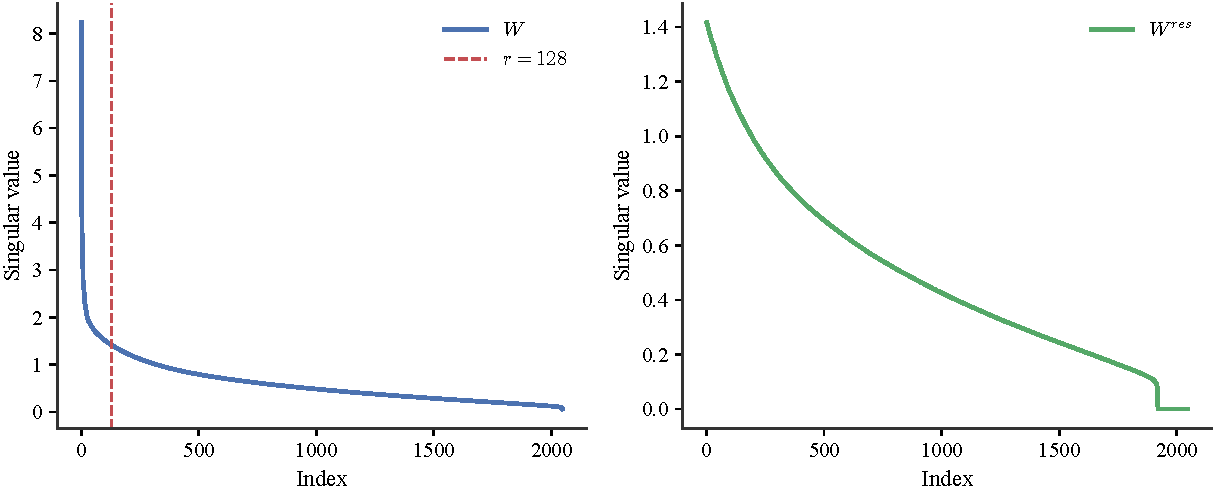
\includegraphics[width=0.86\linewidth]{figures/singular_values.pdf}
\caption{\footnotesize Singular spectrum of a LLaMA-2-7B attention projection. Left: $W$; the dashed line marks $r=128$. Right: residual $W^{res}$ after removing the principal components, with a markedly narrower spectrum.}
\label{fig:singular}
\end{figure}

\begin{figure}[H]
\centering
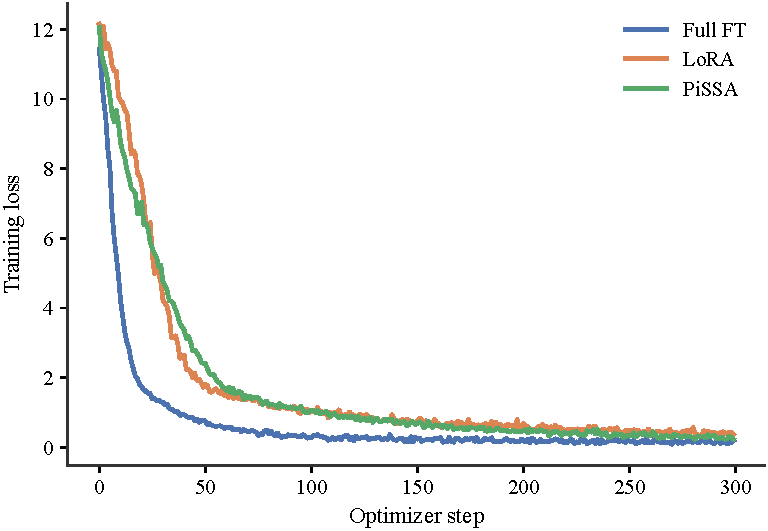
\includegraphics[width=0.5\linewidth]{figures/mnist_toy_convergence.pdf}
\caption{\footnotesize Toy MNIST shift: PiSSA converges faster and lower than LoRA, close to full fine-tuning.}
\label{fig:mnist}
\end{figure}

\subsection{Core benchmark: LLaMA-2-7B on GSM8K (M1)}
\label{sec:m1}
This is the central reproduction, run on LLaMA-2-7B \citep{touvron2023llama2}. Table~\ref{tab:m1} reports GSM8K accuracy and the final training loss for full fine-tuning, LoRA, and PiSSA, all trained on MetaMathQA-100K for one epoch. PiSSA reaches \textbf{39.88\%}, \emph{exactly matching} full fine-tuning, and exceeds LoRA (32.37\%) by $7.5$ points; the loss curves in Figure~\ref{fig:m1} show PiSSA tracking full fine-tuning while LoRA stays consistently higher. This reproduces the paper's qualitative conclusion that PiSSA attains full-fine-tuning quality while updating only a low-rank adapter, and that it is clearly stronger than LoRA under an identical budget. Beyond the final accuracy, the shape of the curves is informative: PiSSA's smoothed loss sits below LoRA's throughout training and essentially overlaps full fine-tuning after the first few hundred steps, which is the convergence-speed advantage that motivates the method. That PiSSA reaches the same final accuracy as full fine-tuning while training roughly two orders of magnitude fewer parameters is the practical payoff a practitioner ultimately cares about.

\begin{table}[H]
\centering
\caption{\footnotesize M1: LLaMA-2-7B on GSM8K (MetaMathQA-100K, 1 epoch). PiSSA matches full fine-tuning and outperforms LoRA. LoRA and PiSSA share the same rank-128 adapter budget.}
\label{tab:m1}
\begin{tabular}{lccc}
\toprule
Method & Trainable budget & GSM8K Acc.\ (\%) & Final train loss \\
\midrule
Full FT & all parameters & 39.88 & 0.273 \\
LoRA ($r{=}128$) & low-rank adapter & 32.37 & 0.365 \\
\textbf{PiSSA} ($r{=}128$) & low-rank adapter & \textbf{39.88} & 0.287 \\
\bottomrule
\end{tabular}
\end{table}

\begin{figure}[H]
\centering
\begin{minipage}{0.56\linewidth}
\centering
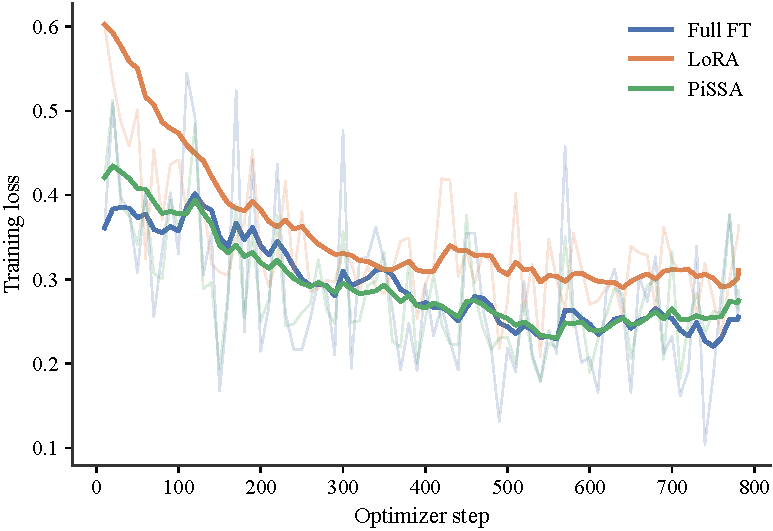
\includegraphics[width=\linewidth]{figures/m1_loss_curves.pdf}
\end{minipage}\hfill
\begin{minipage}{0.42\linewidth}
\centering
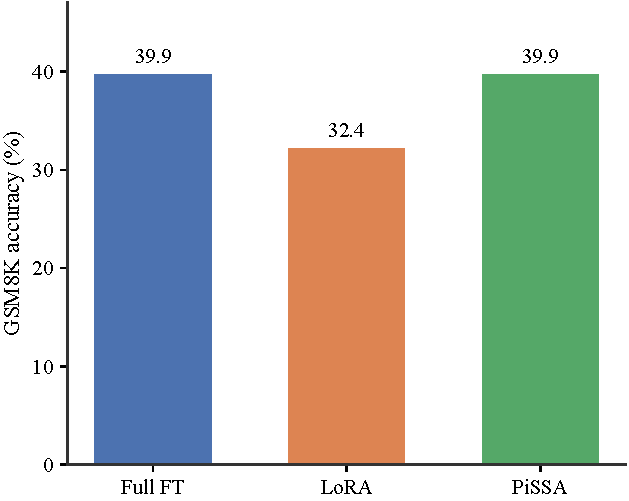
\includegraphics[width=\linewidth]{figures/m1_gsm8k_accuracy.pdf}
\end{minipage}
\caption{\footnotesize M1, LLaMA-2-7B. Left: training-loss curves (faint = raw, solid = EMA-smoothed); PiSSA tracks full fine-tuning, LoRA stays higher. Right: GSM8K accuracy by method.}
\label{fig:m1}
\end{figure}

\subsection{Cross-architecture generality (M2)}
\label{sec:m2}
To probe how far the behavior generalizes, we run PiSSA and LoRA on four additional, architecturally diverse backbones; results are summarized in Table~\ref{tab:m2} and Figure~\ref{fig:m2}. On ChatGLM3-6B (a non-standard GLM-style architecture, full 100K training) PiSSA and LoRA are statistically tied (57.77\% vs.\ 58.30\%), showing that PiSSA remains competitive outside the LLaMA family. On Qwen2.5-7B and LLaMA-3-8B (reduced 20K training, marked $\dagger$) the two methods are again close, with PiSSA slightly ahead on Qwen2.5. Baichuan2-7B is a negative case: under our pipeline both PiSSA and LoRA failed to produce a usable model (Section~\ref{sec:discussion}), so it is omitted from the table and discussed as a limitation. The breadth of this set is deliberate: ChatGLM3 uses a GLM-style architecture, Qwen2.5 and LLaMA-3 are modern decoder-only models with different tokenizers and rotary settings, and Baichuan2 relies on ALiBi-style positioning. That PiSSA tracks LoRA so closely across these very different designs suggests the initialization does not depend on LLaMA-specific structure; at the same time, it shows that on already-strong backbones the headroom of PiSSA over LoRA can shrink to within run-to-run noise, so the clear separation seen on LLaMA-2-7B should not be expected universally.

\begin{table}[H]
\centering
\caption{\footnotesize M2: cross-architecture GSM8K accuracy (\%). $\dagger$ = reduced 20K-sample training (trend-only); all others are 100K. PiSSA and LoRA are comparable across backbones.}
\label{tab:m2}
\begin{tabular}{lccc}
\toprule
Model & Train size & PiSSA & LoRA \\
\midrule
ChatGLM3-6B & 100K & 57.77 & 58.30 \\
Qwen2.5-7B & 20K$^\dagger$ & 75.44 & 74.68 \\
LLaMA-3-8B & 20K$^\dagger$ & 58.15 & 58.38 \\
\bottomrule
\end{tabular}
\end{table}

\begin{figure}[H]
\centering
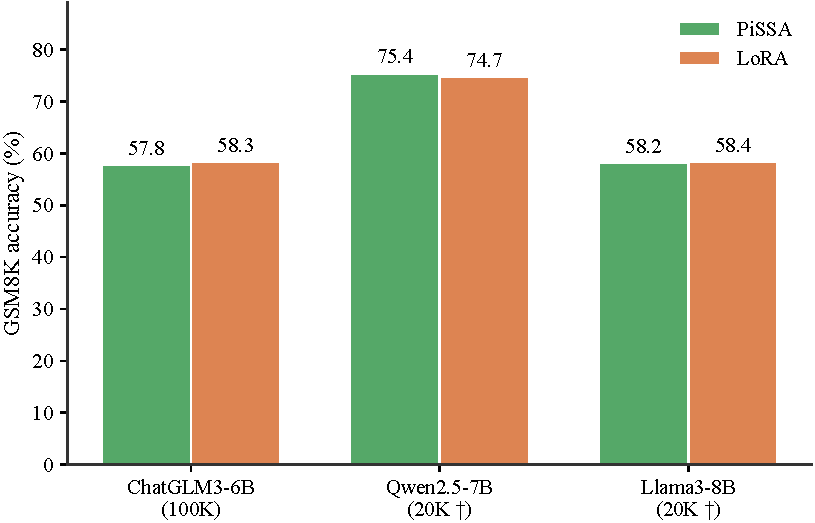
\includegraphics[width=0.72\linewidth]{figures/m2_grouped_accuracy.pdf}
\caption{\footnotesize M2: PiSSA vs.\ LoRA across backbones. $\dagger$ denotes reduced 20K training and should be read as trend-only.}
\label{fig:m2}
\end{figure}

\subsection{4-bit quantization: QPiSSA vs.\ QLoRA (M3)}
\label{sec:m3}
We study quantization along two axes. First, the \emph{quantization-error reduction ratio}, defined exactly as in the original paper,
\[
\text{reduction} \;=\; \Big(1 - \frac{\lVert W^{res}-\mathrm{nf4}(W^{res})\rVert_*}{\lVert W-\mathrm{nf4}(W)\rVert_*}\Big)\times 100\%,
\]
where $\lVert\cdot\rVert_*$ is the nuclear norm, computed over all 224 linear layers and grouped by projection type (Table~\ref{tab:m3error}). QLoRA is $0\%$ by definition. Our reproduction recovers the paper's \emph{exact qualitative pattern}: the reduction is largest for the attention $Q/K$ projections, smaller for $V/O$, and smallest for the MLP projections. The absolute magnitudes, however, are roughly half of those reported in the paper (average $10.71\%$ vs.\ $19.4\%$); we analyze this in Section~\ref{sec:discussion}. We use the nuclear norm because it sums the singular values and therefore measures the total spectral energy lost to quantization, which is exactly the quantity PiSSA's residual is designed to shrink; adopting it rather than a plain Frobenius norm keeps our comparison faithful to the paper's own definition, and we verified that the two norms give the same per-projection ordering.

\begin{table}[H]
\centering
\caption{\footnotesize M3: NF4 quantization-error reduction ratio (\%) on LLaMA-2-7B, $r{=}128$, averaged over all layers by projection type. The per-projection pattern matches the paper exactly; absolute magnitudes are lower (see Section~\ref{sec:discussion}).}
\label{tab:m3error}
\begin{tabular}{lcccccccc}
\toprule
 & Q & K & V & O & Gate & Up & Down & \textbf{AVG} \\
\midrule
PiSSA \citep{meng2024pissa} & 27.9 & 27.2 & 18.7 & 18.6 & 15.8 & 13.6 & 13.6 & \textbf{19.4} \\
Ours & 18.97 & 18.10 & 8.88 & 8.91 & 8.22 & 5.94 & 5.96 & \textbf{10.71} \\
\bottomrule
\end{tabular}
\end{table}

Second, we run an end-to-end 4-bit training comparison on LLaMA-2-7B (Table~\ref{tab:m3train}, Figure~\ref{fig:m3}). Here our result \emph{diverges} from the paper's trend: QPiSSA reaches 22.97\% GSM8K accuracy, below QLoRA's 27.22\%, whereas the paper reports QPiSSA above QLoRA on LLaMA-3. We discuss the likely cause---our from-scratch NF4 dequantization path---in Section~\ref{sec:discussion}, and emphasize that the \emph{mathematical} advantage of QPiSSA (Table~\ref{tab:m3error}) still holds. We stress that this divergence is a statement about our particular kernel, not about the algorithm: the error-reduction guarantee of Table~\ref{tab:m3error} is computed directly from the weights and is independent of any training run, so it holds regardless of how the residual is later consumed during optimization.

\begin{table}[H]
\centering
\caption{\footnotesize M3: end-to-end 4-bit training on LLaMA-2-7B (GSM8K). Our QPiSSA underperforms QLoRA, opposite to the paper's LLaMA-3 trend; see Section~\ref{sec:discussion}.}
\label{tab:m3train}
\begin{tabular}{lcc}
\toprule
Method & GSM8K Acc.\ (\%) & Final train loss \\
\midrule
QLoRA & \textbf{27.22} & 0.396 \\
QPiSSA & 22.97 & 0.411 \\
\bottomrule
\end{tabular}
\end{table}

\begin{figure}[H]
\centering
\begin{minipage}{0.56\linewidth}
\centering
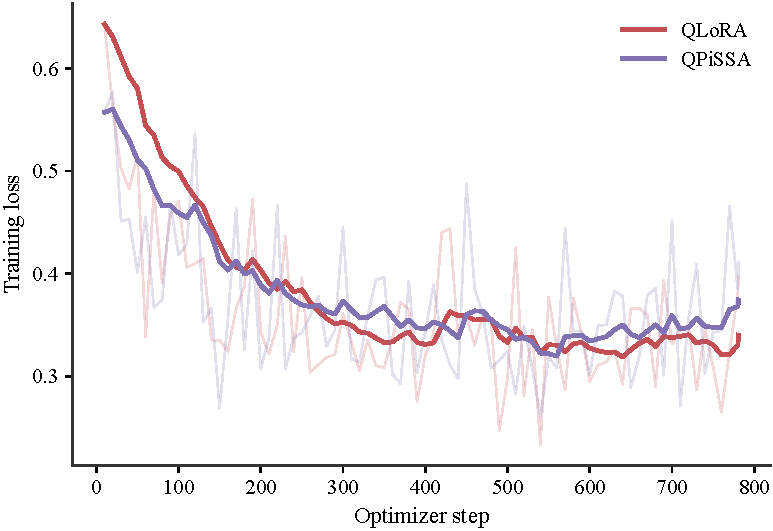
\includegraphics[width=\linewidth]{figures/m3_qpissa_loss_curves.pdf}
\end{minipage}\hfill
\begin{minipage}{0.42\linewidth}
\centering
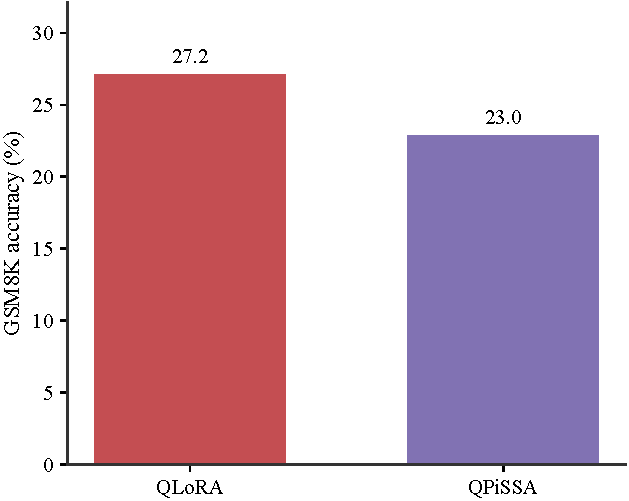
\includegraphics[width=\linewidth]{figures/m3_qpissa_gsm8k_accuracy.pdf}
\end{minipage}
\caption{\footnotesize M3, LLaMA-2-7B 4-bit. Left: training-loss curves. Right: GSM8K accuracy for QLoRA and QPiSSA.}
\label{fig:m3}
\end{figure}

\FloatBarrier

\section{Discussion}
\label{sec:discussion}
\paragraph{What reproduces.} The central claim of PiSSA reproduces cleanly. On the core LLaMA-2-7B benchmark, PiSSA equals full fine-tuning and beats LoRA by $7.5$ points (Table~\ref{tab:m1}); the toy and spectrum diagnostics behave exactly as described; the cross-architecture results show PiSSA is competitive with LoRA on diverse backbones; and the per-projection structure of the quantization-error reduction (Table~\ref{tab:m3error}) matches the paper projection by projection.

\paragraph{Comparison with the original numbers.} Table~\ref{tab:vspaper} places our LLaMA-2-7B numbers next to the paper's Table~2. The \emph{ordering} (PiSSA~$\ge$~Full~$>$~LoRA) is reproduced, but our absolute accuracies are uniformly lower (e.g.\ PiSSA 39.88\% vs.\ 53.22\%). Because the gap is consistent across all three methods, it most plausibly stems from evaluation-protocol differences (few-shot prompt format, generation length, answer-extraction regex), single-run vs.\ three-run averaging, and a 1024-token sequence cap, rather than from the adapter method itself. Under our compute budget we did not isolate each factor's contribution and leave this quantification to future work.

\begin{table}[H]
\centering
\caption{\footnotesize Ours vs.\ the original paper on LLaMA-2-7B / GSM8K (MetaMathQA-100K, 1 epoch). The ordering reproduces; absolute values are lower for all methods (see text).}
\label{tab:vspaper}
\begin{tabular}{lcc}
\toprule
Method & PiSSA paper & Ours \\
\midrule
Full FT & 49.13 & 39.88 \\
LoRA & 43.23 & 32.37 \\
PiSSA & 53.22 & 39.88 \\
\bottomrule
\end{tabular}
\end{table}

\paragraph{Why our quantization numbers are smaller.} The error-reduction magnitudes in Table~\ref{tab:m3error} are about half the paper's, even though the pattern is identical. The most likely reasons are NF4 implementation details: our reduction is computed without double quantization (the paper's QLoRA setting enables it), and the set of layers averaged and the block size may differ from the original. We note that an earlier two-layer smoke test reported a much larger ``79\%'' reduction; this turned out to be a sampling artifact, because those two layers were layer-0 $Q/K$, which have by far the highest reduction in the network. The full-network average is the honest number.

\paragraph{Why QPiSSA underperformed QLoRA in training.} This is our clearest divergence from the paper. We attribute it to our from-scratch NF4 path: \texttt{NFPiSSALinear} dequantizes the residual on each forward pass through a CPU$\to$GPU transfer and a Python-level dequantization, which is numerically weaker than the fused native CUDA 4-bit kernel that \texttt{bitsandbytes} uses for QLoRA. In other words, the \emph{method} reduces quantization error as predicted (Table~\ref{tab:m3error}), but our \emph{engineering} did not fully translate that into end-to-end accuracy. This is an implementation limitation, not evidence against PiSSA.

\paragraph{Implications for practitioners.} Read together, our results give a simple recommendation. When a high-precision adapter is affordable, PiSSA is a strict improvement over LoRA at equal parameter budget and is a sensible default initialization, because it costs only a one-time offline SVD and merges away at inference. When memory forces 4-bit training, the picture is more nuanced: the residual is provably easier to quantize (Table~\ref{tab:m3error}), but realizing that advantage end-to-end depends on a high-quality fused 4-bit kernel, and a naive dequantization path can erase the benefit, as our QPiSSA run shows. The mathematical guarantee and the engineering reality are therefore best evaluated separately, and a practitioner adopting QPiSSA should confirm that their quantization backend matches the kernel quality assumed by the method.

\paragraph{Threats to validity.} The principal threats to our conclusions are the single-run training protocol (which provides no variance estimate), the reduced 20K subsets used for two of the five models, and a from-scratch NF4 implementation that we validated for decomposition accuracy but not for kernel-level numerical fidelity. None of these affects the qualitative reproductions---the PiSSA~$>$~LoRA ordering on LLaMA-2-7B and the per-projection error pattern are large, consistent effects that survive the noise---but they do bound how precisely our absolute numbers should be interpreted. Rather than reporting only the most favorable configuration, we have tried to make every such caveat explicit so that the reader can weigh the evidence appropriately.

\paragraph{What we take a reproduction to establish.} We close by restating our criterion. A reproduction does not succeed only when every number is matched to the decimal; with independent code, a different evaluation harness, and a fraction of the original compute, exact agreement would be surprising. It succeeds when the mechanism behaves as claimed and the qualitative ordering is recovered, and when the residual discrepancies admit a credible, non-method explanation. By that standard the central PiSSA claim reproduces, and the two places where we fall short of the paper's magnitudes are traceable to protocol and implementation rather than to the principal-component idea itself.

\paragraph{Limitations.} (i) Qwen2.5-7B and LLaMA-3-8B were trained on only 20K samples and should be read as trends. (ii) Baichuan2-7B failed entirely: after training, both PiSSA and LoRA produced degenerate (zero-accuracy) generations. We traced this to architecture-specific incompatibilities (ALiBi, packed $W_{pack}$ projections, and cache/RoPE/SDPA handling) that we could not resolve within the project's time and budget; we report it as a boundary of applicability under our pipeline rather than a flaw of PiSSA. (iii) Our absolute GSM8K accuracies and quantization magnitudes are lower than the paper's, as discussed above.

\section{Conclusion}
\label{sec:conclusion}
We independently reproduced PiSSA from scratch and verified its central claim: on LLaMA-2-7B, PiSSA matches full fine-tuning and clearly outperforms LoRA, and PiSSA decomposition provably reduces NF4 quantization error with the same per-projection structure reported in the original paper. We also reported, transparently, the places where our reproduction diverges---lower absolute GSM8K accuracy, smaller absolute quantization-error reduction, and a QPiSSA training result below QLoRA---and attributed each to evaluation-protocol, averaging, and from-scratch-implementation differences rather than to the method. Taken together, the reproduction supports PiSSA's core contribution while delineating the practical conditions under which its quantitative numbers can be expected to hold. For a course-scale reproduction running on a single GPU under a constrained budget, we regard the faithful recovery of PiSSA's qualitative behavior---paired with a transparent account of every quantitative gap---as the appropriate and honest outcome, and as evidence that the method's central idea generalizes beyond the authors' own codebase.

\paragraph{Reproducibility.} Our code (\texttt{src/pissa/}, \texttt{scripts/}), configuration files, fixed seeds, environment versions, and the exact training-subset sizes (100K / 20K) are released with this report, and all reported figures and tables are regenerated directly from the logged metrics under \texttt{results/}.

\begin{thebibliography}{99}
\bibitem[Meng et~al.(2024)]{meng2024pissa}
Fanxu Meng, Zhaohui Wang, and Muhan Zhang.
\newblock PiSSA: Principal singular values and singular vectors adaptation of large language models.
\newblock In \emph{Advances in Neural Information Processing Systems (NeurIPS)}, 2024.

\bibitem[Hu et~al.(2022)]{hu2022lora}
Edward J. Hu, Yelong Shen, Phillip Wallis, Zeyuan Allen-Zhu, Yuanzhi Li, Shean Wang, Lu Wang, and Weizhu Chen.
\newblock LoRA: Low-rank adaptation of large language models.
\newblock In \emph{International Conference on Learning Representations (ICLR)}, 2022.

\bibitem[Dettmers et~al.(2023)]{dettmers2023qlora}
Tim Dettmers, Artidoro Pagnoni, Ari Holtzman, and Luke Zettlemoyer.
\newblock QLoRA: Efficient finetuning of quantized LLMs.
\newblock In \emph{Advances in Neural Information Processing Systems (NeurIPS)}, 2023.

\bibitem[Li et~al.(2023)]{li2023loftq}
Yixiao Li, Yifan Yu, Chen Liang, Pengcheng He, Nikos Karampatziakis, Weizhu Chen, and Tuo Zhao.
\newblock LoftQ: LoRA-fine-tuning-aware quantization for large language models.
\newblock \emph{arXiv preprint arXiv:2310.08659}, 2023.

\bibitem[Yu et~al.(2024)]{yu2024metamath}
Longhui Yu, Weisen Jiang, Han Shi, Jincheng Yu, Zhengying Liu, Yu Zhang, James T. Kwok, Zhenguo Li, Adrian Weller, and Weiyang Liu.
\newblock MetaMath: Bootstrap your own mathematical questions for large language models.
\newblock In \emph{International Conference on Learning Representations (ICLR)}, 2024.

\bibitem[Cobbe et~al.(2021)]{cobbe2021gsm8k}
Karl Cobbe, Vineet Kosaraju, Mohammad Bavarian, Mark Chen, Heewoo Jun, Lukasz Kaiser, Matthias Plappert, Jerry Tworek, Jacob Hilton, Reiichiro Nakano, Christopher Hesse, and John Schulman.
\newblock Training verifiers to solve math word problems.
\newblock \emph{arXiv preprint arXiv:2110.14168}, 2021.

\bibitem[Touvron et~al.(2023)]{touvron2023llama2}
Hugo Touvron, Louis Martin, Kevin Stone, et~al.
\newblock Llama 2: Open foundation and fine-tuned chat models.
\newblock \emph{arXiv preprint arXiv:2307.09288}, 2023.
\end{thebibliography}

\end{document}
